%
% File: chap01.tex
%
\let\textcircled=\pgftextcircled
\chapter{Reactor Heat Generation}
\label{chap:intro}

\initial{S}everal exercises from the book written by M. M. El Wakil~\cite{book01} are tackled in this homework. The problems in this section relate to the seventh and eigth chapter of the book, covering the subject of heat conduction in reactor elements.

%=======
\section{[7-6] - Rectangular fin}
\label{prob71}

\subsection{Problem}
\textit{A very long fin is rectangular in cross-section $0.48 * 0.24$ in. It generates \num{2e6} $Btu.h^{-1}.ft^{-3}$. The fin base is at $1000{}^\circ F$. It is cooled by a gas at $600{}^\circ F$ with a uniform heat transfer coefficient $100\ Btu.h^{-1}.ft^{-2}.{}^\circ F^{-1}$. Using a network with $\Delta x = 0.12$ in., write the necessary set of finite difference equations for the nodal points and solve by any one of the techniques at your command. $k$ for the fin material $= 10\ Btu.h^{-1}.ft^{-1}.{}^\circ F^{-1}$}

\subsection{Solution}

First, one can note that the problem is missing a graph. The considered geometry is given in Figure~\ref{fig71}.

\begin{figure}[H]
\centering
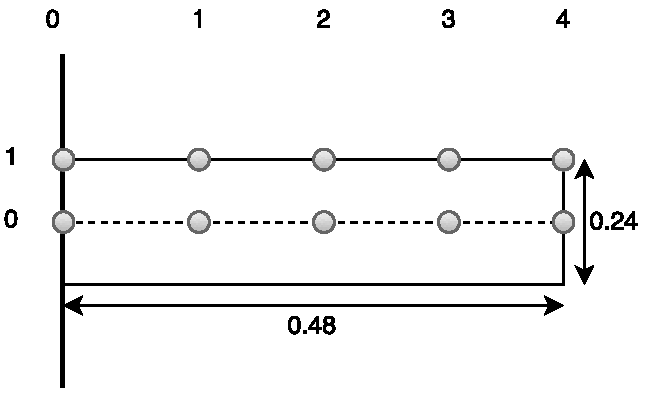
\includegraphics[scale=1]{fig/schema.pdf}
\caption{Representation of the problem geometry}
\label{fig71}
\end{figure}

We can identify four types of nodes: inner, y-bound (next to the upper boundary), x-bound (next to the right boundary) and corner.

The inner node temperature $T_n$ is given by Equation~\ref{eq71}.

\begin{equation}\label{eq71}
T_n = \frac{T_{n-\Delta x} + T_{n+\Delta x} + T_{n-\Delta y} + T_{n+\Delta y}}{4} + \frac{\Delta T_g}{2}
\end{equation}

In our case, we can see that $T_{n-\Delta y} = T_{n+\Delta y}$ by symmetry for the inner nodes. Consequently, we obtain Equation~\ref{eq72}.

\begin{equation}\label{eq72}
T_n = \frac{T_{n-\Delta x} + T_{n+\Delta x} + 2T_{n+\Delta y}}{4} + \frac{\Delta T_g}{2}
\end{equation}

For the x-bound nodes, we can write Equation~\ref{eq73}.


\begin{equation}\label{eq73}
T_n = \frac{T_{n-\Delta x} + T_{n+\Delta y} + Bi_{\Delta x}T_f}{2 + 2Bi_{\Delta x}} + \frac{\Delta T_g}{2+Bi_{\Delta x}}
\end{equation}

For the y-bound nodes, we can write Equation~\ref{eq74}

\begin{equation}\label{eq74}
T_n = \frac{T_{n-\Delta x} + T_{n+\Delta x} + 2T_{n+\Delta y} + 2Bi_{\Delta x}T_f}{4 + 2Bi_{\Delta x}} + \frac{\Delta T_g}{2+Bi_{\Delta x}}
\end{equation}

And finally, for the corner node, we can write (as seen in problem 7.1 previously) Equation~\ref{eq75}.

\begin{equation}\label{eq75}
T_n = \frac{T_{n-\Delta x} + T_{n+\Delta y} + 2Bi_{\Delta x}T_f}{2 + 2Bi_{\Delta x}} + \frac{\Delta T_g}{2+2Bi_{\Delta x}}
\end{equation}

A few exceptions can be noted. Indeed, the two leftmost points, on the base of the fin, are given to be at $1000{}^\circ F$.

We can consequently write the matrix $A$. 


\setcounter{MaxMatrixCols}{30}
\tiny
\[
A =
  \begin{bmatrix}
1     & 0    & 0     & 0     & 0     & 0     & 0     & 0     & 0     & 0          \\
0     & 1    & 0     & 0     & 0     & 0     & 0     & 0     & 0     & 0          \\
-0.25 & 0    & 1     & -0.5  & -0.25 & 0     & 0     & 0     & 0     & 0          \\
0     & \frac{-1}{2Bi_{\Delta x}+4}     & \frac{-1}{Bi_{\Delta x}+2} & 1 & 0     & \frac{-1}{2Bi_{\Delta x}+4}  & 0 & 0     & 0     & 0          \\
0 & 0 & -0.25 & 0    & 1     & -0.5  & -0.25 & 0     & 0     & 0           \\
0 & 0 & 0     & \frac{-1}{2Bi_{\Delta x}+4}     & \frac{-1}{Bi_{\Delta x}+2} & 1 & 0     & \frac{-1}{2Bi_{\Delta x}+4}  & 0 & 0           \\
0 & 0 & 0 & 0 & -0.25 & 0    & 1     & -0.5  & -0.25 & 0            \\
0 & 0 & 0 & 0 & 0     & \frac{-1}{2Bi_{\Delta x}+4}     & \frac{-1}{Bi_{\Delta x}+2} & 1 & 0     & \frac{-1}{2Bi_{\Delta x}+4}           \\
0 & 0 & 0 & 0 & 0     & 0 & \frac{-1}{Bi_{\Delta x}+2} & 0 & 1 & \frac{-1}{Bi_{\Delta x}+2} \\
0 & 0 & 0 & 0 & 0     & 0 & 0 & \frac{-1}{2Bi_{\Delta x}+2} & \frac{-1}{2Bi_{\Delta x}+2} & 1 \\
  \end{bmatrix}
\]

\normalsize

$\frac{\Delta T_g}{2}$ can be calculated using $\Delta T_g = \frac{(\Delta x)^2 q'''}{2k}$. $T_f$, the temperature of the gas, is known. We can thus obtain $b$.
\tiny
\[
b =
  \begin{bmatrix}
1000 \\
1000 \\
7.2 \\
229.5\\
7.2\\
229.5\\
7.2 \\
229.5\\
229.5\\
330.5\\
   \end{bmatrix}
\]

\normalsize

The equation $A.x = b$ can thus be solved, using Python. The python script is given in~\ref{py1}. We obtain the following results (Equation~\ref{eq76}):

\begin{equation}\label{eq76}
\begin{aligned}
T(0,0) = 1000.0 \\
T(0,1) = 1000.0 \\
T(1,0) = 804.0 \\
T(1,1) = 740.9\\
T(2,0) = 705.3\\
T(2,1) = 665.0\\
T(3,0) = 658.5\\
T(3,1) = 635.7\\
T(4,0) = 628.3\\
T(4,1) = 617.8\\
\end{aligned}
\end{equation}


\newpage
\subsubsection{Python script}
\label{py1}
\begin{lstlisting}[language=python]
import numpy as np

m = 10    # size of system is m x m

dx = 0.12
deltax, k, qtriple, h = (dx/10)**2, 10., 2.e6, 100.    # BG units
tb = 1000.
ts = 600.
dtg = (0.5*deltax)*qtriple/k
bi = h * dx / k

amat = np.zeros((m,m))
b = np.zeros(m)
    
amat[0,0] = 1.
amat[1,1] = 1.
b[0] = tb
b[1] = tb

for i in range(2, m, 2):
    try:
        amat[i,i-2] = -0.25
        amat[i,i] = 1.
        amat[i,i+1] = -0.5
        amat[i,i+2] = -0.25
        b[i] = dtg/2.
    except IndexError:
        break

for i in range(3, m, 2):
    try:
        amat[i,i-2] = -1/(2*bi+4)
        amat[i,i-1] = -1/(bi+2)
        amat[i,i] = 1.
        amat[i,i+2] = -1/(2*bi+4)
        b[i] = (bi*ts + dtg)/(bi+2)
    except IndexError:
        break

amat[m-1,m-1] = 1.
amat[m-1,m-2] = -1/(2*bi+2)
amat[m-1,m-3] = -1/(2*bi+2)
b[m-1] = (2*bi*ts + dtg)/(2*bi+2)


amat[m-2,m-2] = 1.
amat[m-2,m-1] = -1/(bi+2)
amat[m-2,m-4] = -1/(bi+2)
b[m-2] = (bi*ts + dtg)/(bi+2)
print(b)
ysol = np.linalg.solve(amat,b)

print('Temperature solution:')

temp = []
for i in range(5):
    for j in range(2):
        temp.append("T(%s,%s)" % (i, j))
        
for i,t in enumerate(temp):
    print("%s = %.1f" % (t, ysol[i]))
    
# check of solution: 
if not np.allclose(np.dot(amat, ysol), b):
    print("Solution does not match!")
\end{lstlisting}
\newpage

\section{[7-13] - }
\label{prob72}

\subsection{Problem}
\textit{A long fuel element has a rectangular cross-section $1*2$ in. It generates \num{1e6} $Btu.h^{-1}.ft^{-3}$ and has a thermal conductivity of $1.085\ Btu.h^{-1}.ft^{-1}.{}^\circ F^{-1}$. All surfaces are held at $1000{}^\circ F$. Find the heat flux, $Btu.h^{-1}.ft^{-2}$ at the center point of each side using the approximate analytical solution of section 7-13.}

\subsection{Solution}

The book~\cite{book01} gives us a solution for a long rectangular fuel element (Equations 7-34 to 7-44). It is given here by Equation~\ref{eq77}.

\begin{equation}\label{eq77}
T(x,y) = \frac{3}{4}\frac{q'''}{k(a^2+b^2)}(a^2-x^2)(b^2-y^2)
\end{equation}

However, this solution is obtained for different boundary conditions ($T_s = 0{}^\circ F$). In our case, $T_s = 1000{}^\circ F$. Then, we can rewrite Equation~\ref{eq77} to Equation~\ref{eq78} to account for this different boundary condition.


\begin{equation}\label{eq78}
T(x,y) = \frac{3}{4}\frac{q'''}{k(a^2+b^2)}(a^2-x^2)(b^2-y^2) + 1000 = C(a^2-x^2)(b^2-y^2) + 1000
\end{equation}

The heat flux is given in the x-direction by Equation~\ref{eq79} and in the y-direction by Equation~\ref{eq710}.


\begin{equation}\label{eq79}
q''_x = -k\frac{\partial T}{\partial x}
\end{equation}

\begin{equation}\label{eq710}
q''_y = -k\frac{\partial T}{\partial y}
\end{equation}

Consequently, we can write Equations~\ref{eq711} and~\ref{eq712}.

\begin{equation}\label{eq711}
q''_x = -2kCx(y^2-b^2)
\end{equation}

\begin{equation}\label{eq712}
q''_y = -2kCy(x^2-a^2)
\end{equation}

At the center point of each side, we have Equations~\ref{eq713} and~\ref{eq714}.

\begin{equation}\label{eq713}
q''_x\bigg\rvert_{x=a, y=0} = 2kCab^2
\end{equation}

\begin{equation}\label{eq714}
q''_y\bigg\rvert_{x=0, y=b} = 2kCba^2
\end{equation}

So, we obtain $q''_x = \text{\num{2.5e4}}\ Btu.h^{-1}.ft^{-2}$ and $q''_y = \text{\num{5.0e4}}\ Btu.h^{-1}.ft^{-2}$.
